%%=============================================================================
%% Methodologie
%%=============================================================================

\chapter{\IfLanguageName{dutch}{Methodologie}{Methodology}}%
\label{ch:methodologie}

%% TODO: In dit hoofstuk geef je een korte toelichting over hoe je te werk bent
%% gegaan. Verdeel je onderzoek in grote fasen, en licht in elke fase toe wat
%% de doelstelling was, welke deliverables daar uit gekomen zijn, en welke
%% onderzoeksmethoden je daarbij toegepast hebt. Verantwoord waarom je
%% op deze manier te werk gegaan bent.
%% 
%% Voorbeelden van zulke fasen zijn: literatuurstudie, opstellen van een
%% requirements-analyse, opstellen long-list (bij vergelijkende studie),
%% selectie van geschikte tools (bij vergelijkende studie, "short-list"),
%% opzetten testopstelling/PoC, uitvoeren testen en verzamelen
%% van resultaten, analyse van resultaten, ...
%%
%% !!!!! LET OP !!!!!
%%
%% Het is uitdrukkelijk NIET de bedoeling dat je het grootste deel van de corpus
%% van je bachelorproef in dit hoofstuk verwerkt! Dit hoofdstuk is eerder een
%% kort overzicht van je plan van aanpak.
%%
%% Maak voor elke fase (behalve het literatuuronderzoek) een NIEUW HOOFDSTUK aan
%% en geef het een gepaste titel.

Dit onderzoek volgt de opzet van een vergelijkende studie met proof-of-concept, aangevuld met literatuuronderzoek en een requirements-analyse binnen een concrete bedrijfscontext. Het doel is om enerzijds het probleem en de oplossingsruimte rond dependencybeheer in kaart te brengen, en anderzijds een apart dashboard-prototype te bouwen en technisch te evalueren binnen een realistische ontwikkelomgeving.

\subsection{Fase 1 - Verdiepende literatuurstudie en probleemverkenning}
\label{sec:fase1}

In de eerste fase van de bachelorproef wordt de probleemcontext verder uitgediept aan de hand van een systematische literatuurstudie rond dependency management, kwetsbare dependencies, technische schuld en bestaande dependencybots. Daarnaast wordt vakliteratuur over AI-agents en workflow-automatisering bestudeerd om na te gaan welke concepten en benaderingen relevant zijn voor een AI-gestuurd dependency-dashboard.

Tijdens deze fase worden ook één of enkele representatieve projecten van het bedrijf geselecteerd en geanalyseerd (projectstructuur, gebruikte technologieën, dependency-ecosystemen, huidige processen rond updates). De belangrijkste deliverables zijn:
\begin{itemize}
    \item een uitgewerkte en geactualiseerde literatuurstudie;
    \item een scherpere probleemomschrijving toegespitst op de gekozen bedrijfscontext en projecten;
    \item een eerste set geïnformeerde hypotheses over de verwachte impact van een AI-gestuurd dependency-dashboard.
\end{itemize}

\subsection{Fase 2 - Requirements-analyse en architectuurontwerp}
\label{sec:fase2}

In de tweede fase wordt eerst een gerichte requirements-analyse uitgevoerd in samenwerking met de co-promotor via interviews en workshops worden functionele en niet-functionele eisen expliciet gemaakt, zoals:
\begin{itemize}
    \item functionele eisen: integratie met GitHub, beheer van projecten en dependencies in het dashboard, detectie van nieuwe versies via publieke registries, analyse en samenvatting van changelogs en release notes, aanduiding van kriticiteit (security, bugfix, feature), prioritering van updates;
    \item niet-functionele eisen: schaalbaarheid, betrouwbaarheid, traceerbaarheid (logging en audittrail), gebruiksvriendelijkheid en onderhoudbaarheid.
\end{itemize}

Op basis van deze requirements wordt vervolgens een systeemarchitectuur ontworpen voor de webapplicatie en de from-scratch ontworpen AI-agent. De architectuur beschrijft onder meer de globale componenten (frontend, backend, databank, integraties met GitHub en registries), de verantwoordelijkheden per component, de datastromen (bijvoorbeeld van dependency-informatie naar AI-analyse en terug naar het dashboard) en de plaats van eventueel ondersteunende workflow- of agentplatformen. Deliverables van fase 2 zijn:
\begin{itemize}
    \item een requirementsdocument met duidelijke prioritering;
    \item een architectuurbeschrijving (diagrammen, componentbeschrijvingen, datamodellen);
    \item een lijst van geselecteerde technologieën en tools, gemotiveerd vanuit de requirements.
\end{itemize}

\subsection{Fase 3 - Implementatie van het proof-of-concept}
\label{sec:fase3}

In fase 3 wordt de ontworpen architectuur omgezet in een werkend proof-of-concept. De kern bestaat uit een aparte webapplicatie (dashboard) waarin per project de gebruikte dependencies worden bijgehouden en verrijkt met informatie uit publieke registries zoals npm. De applicatie werkt vanaf het begin met één of meerdere reële GitHub-repositories van het bedrijf, zodat de proof-of-concept onmiddellijk getest wordt in een realistische context. Dependency-informatie wordt automatisch uit deze repositories gehaald (bijvoorbeeld via repositoryconfiguratiebestanden) en opgeslagen in een centrale databank.

Parallel wordt de AI-agentlaag geïmplementeerd in de backend. In deze fase worden drie concrete AI-agentoplossingen opgezet en geïntegreerd in hetzelfde dashboard: een agent op basis van OpenAI Agent Builder, een workflow met n8n en een agentconfiguratie met Flowise. Elk van deze varianten ontvangt changelog- en release-note-informatie, genereert beknopte samenvattingen en beoordeelt de aard en vermoedelijke impact van updates (bijvoorbeeld beveiligingsfix, bugfix, nieuwe functionaliteit, potentieel brekende wijziging). De frontend visualiseert de status van dependencies, aanbevolen acties en de door de verschillende AI-varianten gegenereerde toelichting. Deliverables van fase 3 zijn:
\begin{itemize}
    \item een werkend prototype van het dashboard met integratie naar GitHub en één dependency-registries;
    \item drie geïmplementeerde AI-agentvarianten (OpenAI Agent Builder, n8n, Flowise) die changelogs en release notes verwerken en samenvatten;
    \item technische documentatie over de implementatie (architectuur, API’s, datamodellen en integratiepunten voor de agents).
\end{itemize}

\subsubsection{Implementatie van de Mastra-agent}
\label{sec:mastra-implementatie}

Voor de eerste AI-integratie in het dashboard wordt gebruikgemaakt van Mastra, een Typescript-framework om AI-agents, tools en workflows te definiëren en te orchestreren. In de proof-of-concept wordt een \texttt{dependencyAgent} opgezet die specifiek is afgestemd op het analyseren van npm-dependency-updates. Deze agent combineert een taalmodel (bijvoorbeeld \texttt{gemini-2.5-flash} of \texttt{gpt-4o-mini}) met een eigen tool \texttt{fetchNpmInfoTool}, die informatie ophaalt uit de npm-registry en bijhorende release notes van Github.

De agent is geconfigureerd met duidelijke instructies en een vast outputformaat, zodat ontwikkelaars snel een gestructureerd overzicht krijgen van nieuwe features, breaking changes, security fixes, deprecations, migratiestappen en een advies of de update veilig is. Onderstaand codefragment toont de definitie van de agent in Mastra:

% \begin{figure}[H]
%   \centering
%   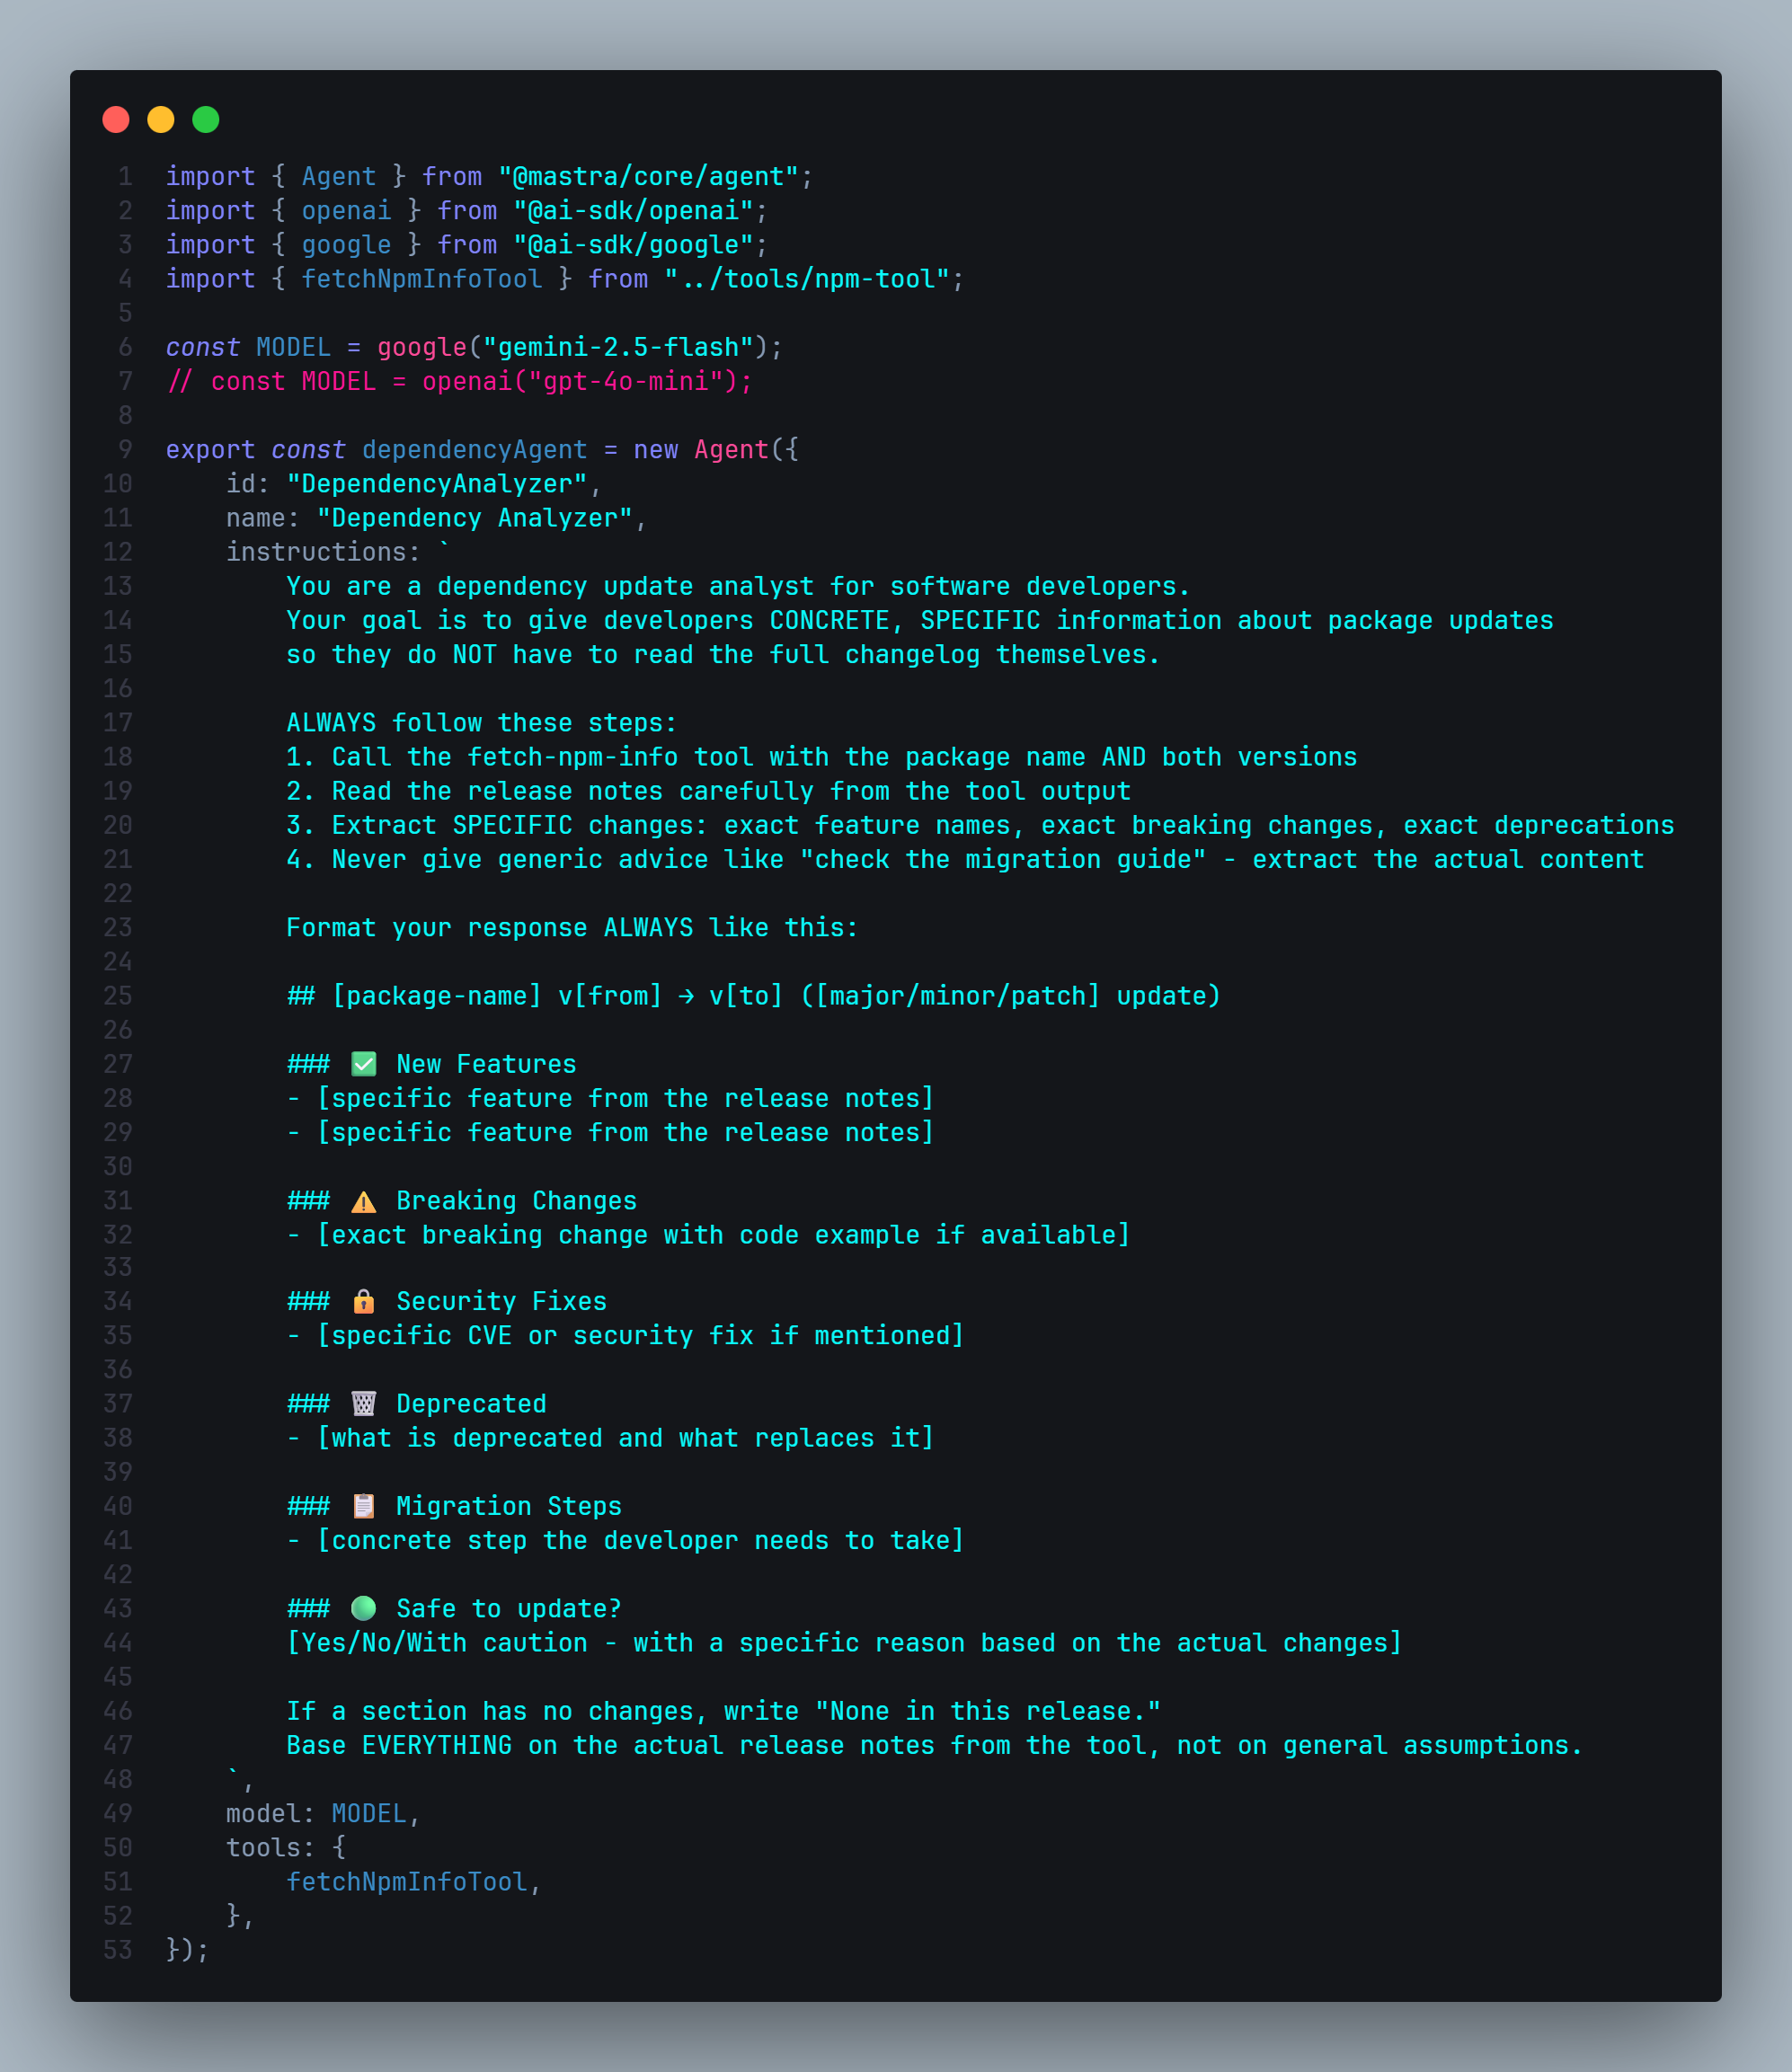
\includegraphics[width=\textwidth,keepaspectratio]{img/dependency-agent.png}
%   \caption[Mastra dependency-agent]{Mastra-agent voor analyse van dependency-updates}
%   \label{fig:mastra-agent-config}
% \end{figure}

De agent maakt gebruik van een custom tool \texttt{fetchNpmInfoTool} om zowel metadata uit de npm-registry als release notes uit Github op te halen. Deze tool accepteert de packagenaam en de versies \texttt{fromVersion} en \texttt{toVersion}, zoekt de repository-URL in de npm-metadata, en probeert vervolgens de relevante GitHub-releases te vinden. Als er geen release is voor de exacte tag, wordt teruggevallen op de laatste releases, zodat de agent steeds over zo volledig mogelijke changelog-informatie beschikt. Het resultaat (beschrijving, homepage, repository en samengestelde \texttt{releaseNotes}) wordt gereialiseerd naar een gestructureerd object waar de agent verder op kan redeneren. De implementatie van de tool is weergegeven in Listing~\ref{lst:mastra-tool}.

% \begin{figure}[H]
%   \centering
%   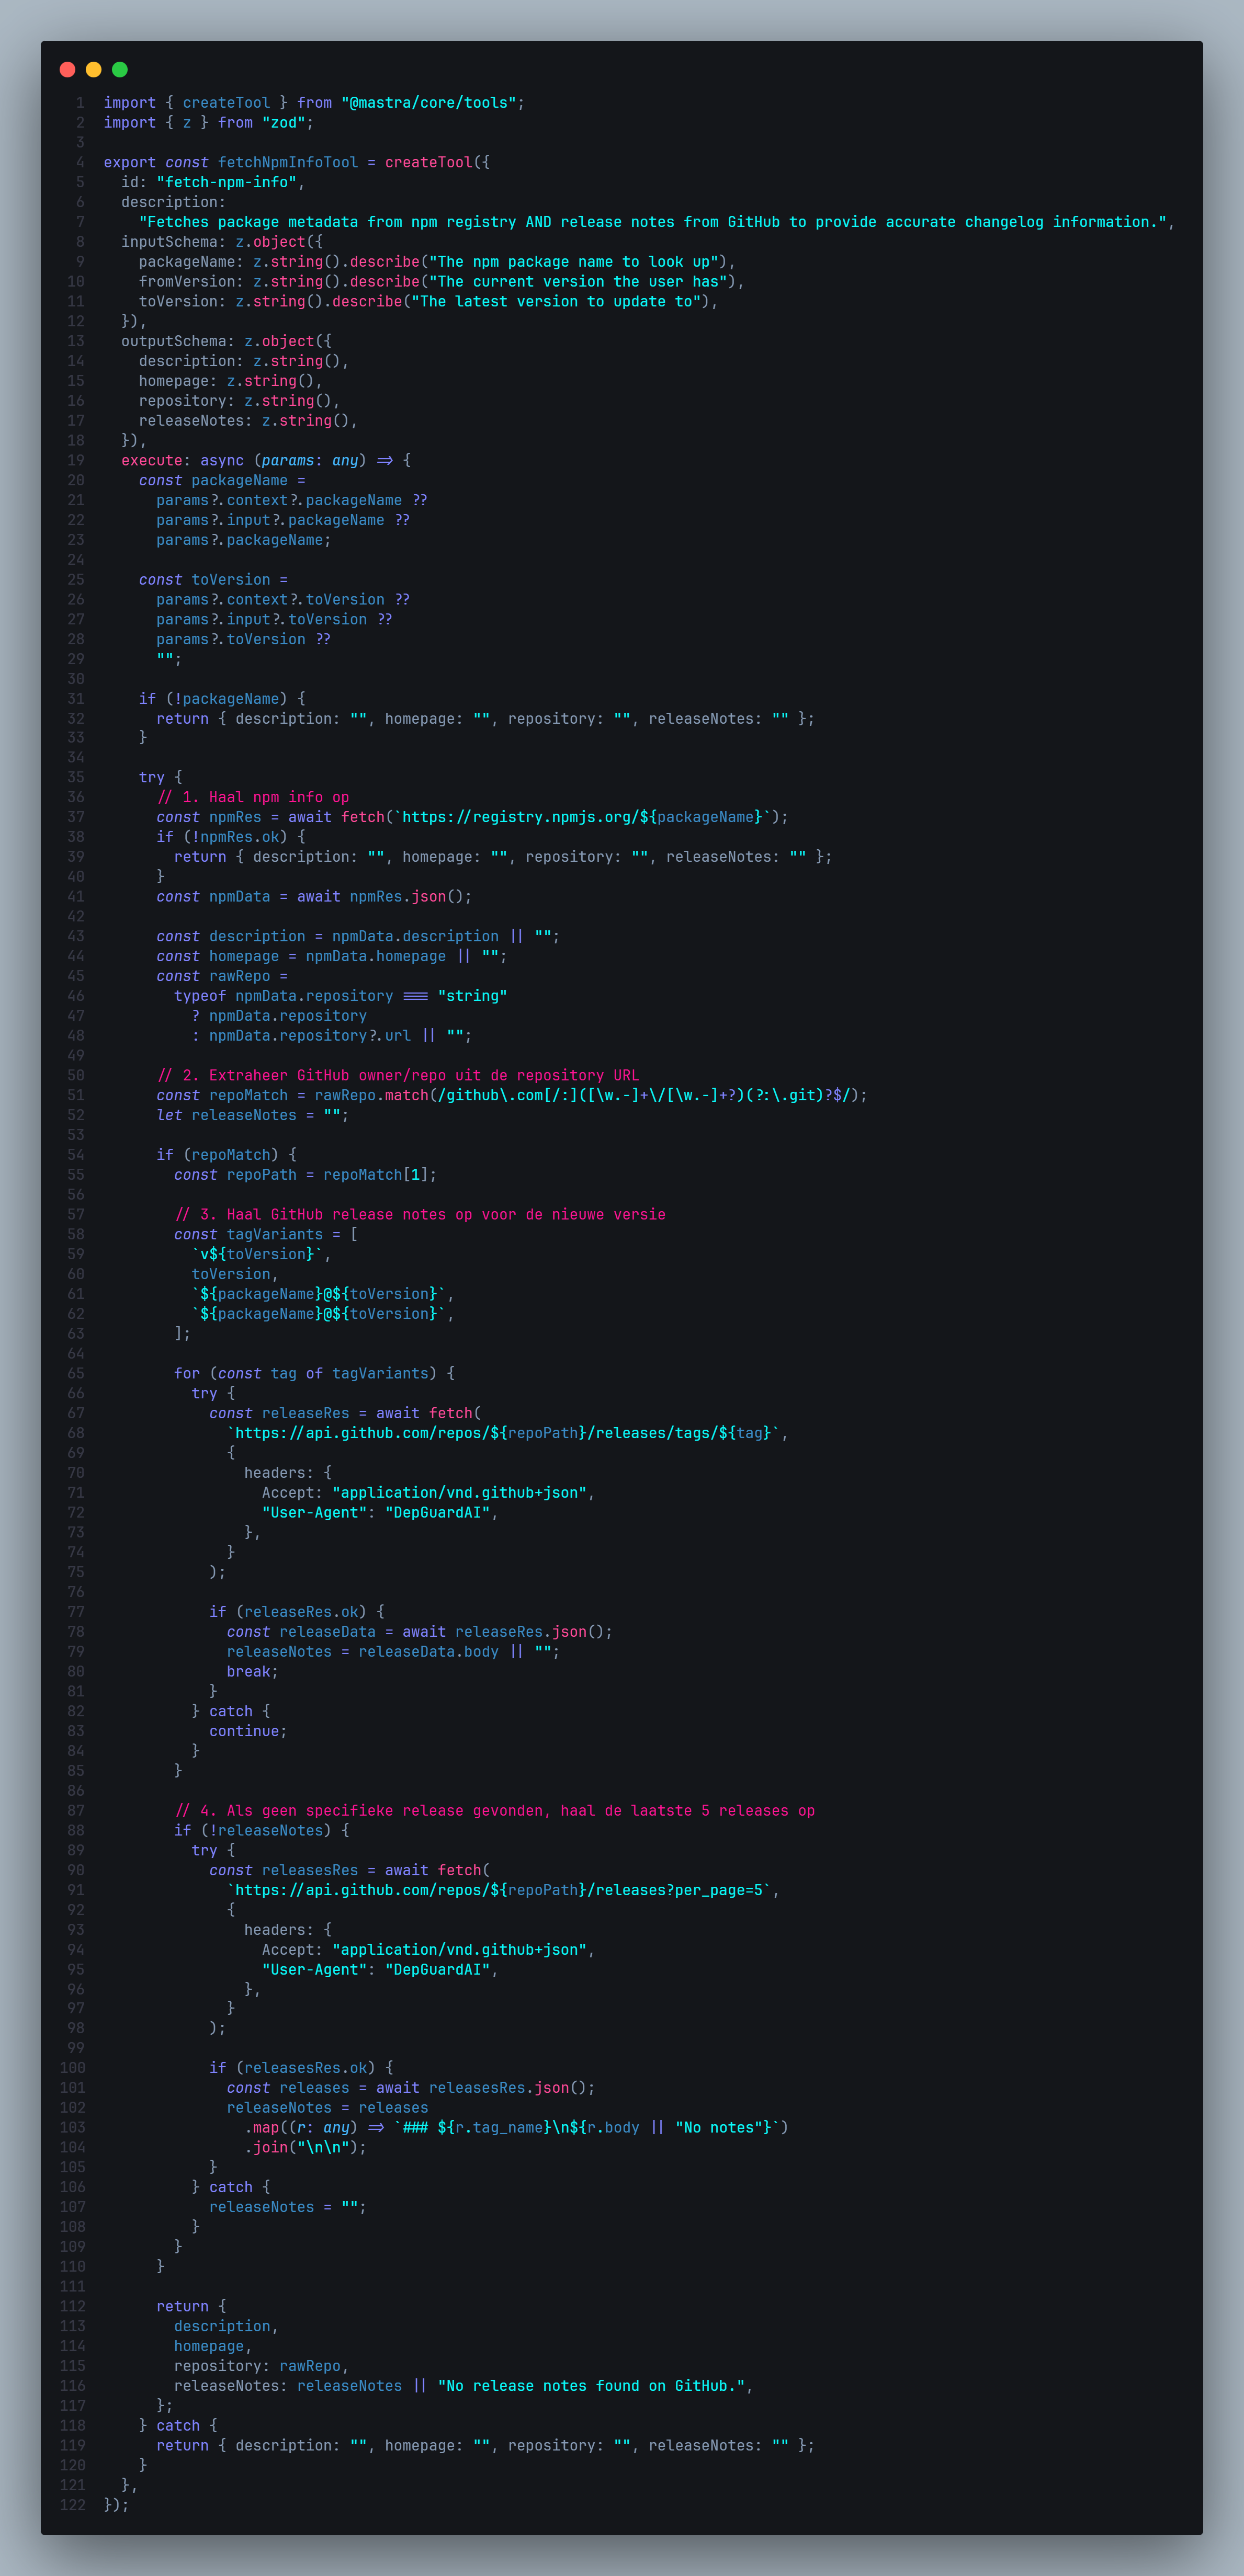
\includegraphics[width=\textwidth,keepaspectratio]{img/npm-tool.png}
%   \caption[Mastra-tool voor npm- en GitHub-informatie]{Tool \texttt{fetchNpmInfoTool} voor het ophalen van npm-metadata en GitHub-release notes}
%   \label{fig:mastra-tool}
% \end{figure}

\subsubsection{Implementatie van de n8n-workflow}
\label{sec:n8n-implementatie}

Als tweede AI-integratie wordt een n8n-workflow opgezet die dezelfde kernfunctie vervult als de Mastra-agent, maar dan in een low-code, visueel georkestreerde omgeving. De workflow ontvangt een HTTP-aanvraag vanuit de webapplicatie, verrijkt de aangeleverde dependency-informatie met data uit npm, Github en een webzoekdienst (Tavily)\footnote{Tavily is een API en infrastructuurlaag die AI-agents en LLM-toepassingen real-time toegang geeft tot webzoekopdrachten, webextractie en crawling.\url{https://www.tavily.com/}}, en laat vervolgens een AI-model (Gemini 2.5 flash) een samenvatting genereren van de relevante wijzigingen. Het resultaat wordt teruggestuurd naar de applicatie via de webhook-respons en opgeslagen in de databank.

De workflow bestaat uit een keten van acht nodes (Figuur~\ref{fig:n8n-workflow}):

\begin{itemize}
    \item \textbf{Node 1: Webhook.} Deze node fungeert als ingangspunt voor de workflow en wordt getriggerd zodra de Next.js-backend een HTTP-aanvraag naar de n8n-URL stuurt. De node is geconfigureerd om te antwoorden via een aparte \emph{Respond to Webhook}-node, zodat alle tussenliggende stappen eerst afgewerkt worden.
    \item \textbf{Node 2: npm-metadata (Code).} In deze code-node wordt de JSON-body van de inkomende request uitgelezen (\texttt{packageName}, \texttt{fromVersion}, \texttt{toVersion}) en wordt via \texttt{this.helpers.httpRequest } een call gedaan naar \texttt{ https://registry.npmjs.org/\{packageName\}}. De node reconstrueert de repository-URL uit de npm-metadata en geeft een nieuwe JSON-object door met omschrijving, homepage en repository-informatie.
    \item \textbf{Node 3: Github-node (Code).} Deze node ontvangt de verrijkte npm-data, extraheert \texttt{owner/repo} uit de repository-URL en probeert via de Github API eerst release notes op te halen voor de specifieke tag (\texttt{v\{toVersion\}} of \texttt{toVersion}). Als die niet gevonden wordt, heelt de node de laatste releases op en concateneert de body-teksten tot een \texttt{releaseNotes}-veld. Als er ook geen releases zijn, wordt er nog geprobeerd een \texttt{CHANGELOG.md}, \texttt{CHANGES.md} of \texttt{HISTORY.md} rechtstreeks uit de repository te lezen. De node voegt \texttt{releaseNotes}, \texttt{changelogUrl} en \texttt{source} toe aan de JSON.
    \item \textbf{Node 4: HTTP Request (Tavily).} Via een HTTP-request-node wordt de Tavily API aangeroeperen om webresultaten op te halen die extra context kunnen geven over de dependency of de update (bijvoorbeeld blogposts of documentatie rond de nieuwe versie).
    \item \textbf{Node 5: Merge-node (Code).} Deze node voegt de Github-data en Tavily-resultaten samen. De webresultaten worden omgezet naar een tekstveld \texttt{webSnippets} (titel, URL en inhoud per resultaat), dat samen met de eerder verzamelde metadata en release notes wordt doorgegeven aan de AI-node.
    \item \textbf{Node 6: AI-agent (Gemini).} Een AI-node, geconfigureerd met het model \texttt{gemini-2.5-flash}, ontvangt \texttt{releaseNotes}, \texttt{webSnippets} en versie-informatie als input. Met behulp van een system prompt en user prompt genereert het model een gestructureerde samenvatting van de update (bijvoorbeeld features, breaking changes, security-aspecten en migratieadvies).
    \item \textbf{Node 7: Code-node (post-processing).} Deze node extraheert de relevante output uit de AI-respons (bijvoorbeeld \texttt{output} of \texttt{summary}) en zet die om naar een eenvoudige JSON-object met één veld \texttt{summary}, zodat de webhook-respons helder en compact blijft.
    \item \textbf{Node 8: Respond to Webhook.} De laatste node stuurt de \texttt{summary} terug als HTTP-respons naar de oorspronkelijke aanroeper. Aan de kant van de webapplicatie kan deze samenvatting vervolgens rechtstreeks worden opgeslagen in de databank.
\end{itemize}

De Next.js-backend roept de n8n-workflow aan via een dedicated route (vereenvoudigd weergegeven in Listing~\ref{lst:n8n-route}). Deze route valideert eerst de gebruiker met Supabase, leest de dependencygegevens uit de inkomende request (\texttt{dependencyId}, \texttt{name}, \texttt{currentVersion}, \texttt{latestVersion}) en stuurt die als JSON-payload door naar de n8n-webhook. De samenvatting die n8n terugstuurt wordt daarna opgeslagen in het veld \texttt{ai\_summary} van de desbetreffende dependency.

\begin{listing}[H]
\begin{minted}{ts}
export async function POST(request: Request) {
  const supabase = await createClient();
  const { data: { user } } = await supabase.auth.getUser();
  if (!user) {
    return NextResponse.json({ error: "Unauthorized" }, { status: 401 });
  }

  const { dependencyId, name, currentVersion, latestVersion } =
    await request.json();

  const n8nRes = await fetch(
    process.env.N8N_WEBHOOK_URL ?? "http://localhost:5678/webhook-test/analyze-dependency",
    {
      method: "POST",
      headers: { "Content-Type": "application/json" },
      body: JSON.stringify({
        packageName: name,
        fromVersion: currentVersion,
        toVersion: latestVersion,
      }),
    }
  );

  const n8nData = await n8nRes.json();
  const summary = n8nData.summary;

  await supabase
    .from("dependencies")
    .update({ ai_summary: summary })
    .eq("id", dependencyId);

  return NextResponse.json({ summary });
}
\end{minted}
\caption[Aanroep van de n8n-workflow]{Next.js-route die de n8n-workflow aanroept en de samenvatting opslaat}
\label{lst:n8n-route}
\end{listing}

Figuur~\ref{fig:n8n-workflow} toont de volledige n8n-workflow zoals geïmplementeerd in deze bachelorproef, met de opeenvolgende nodes van inkomnde webhook tot AI-gegenereerde samenvatting.

\begin{figure}[H]
  \centering
  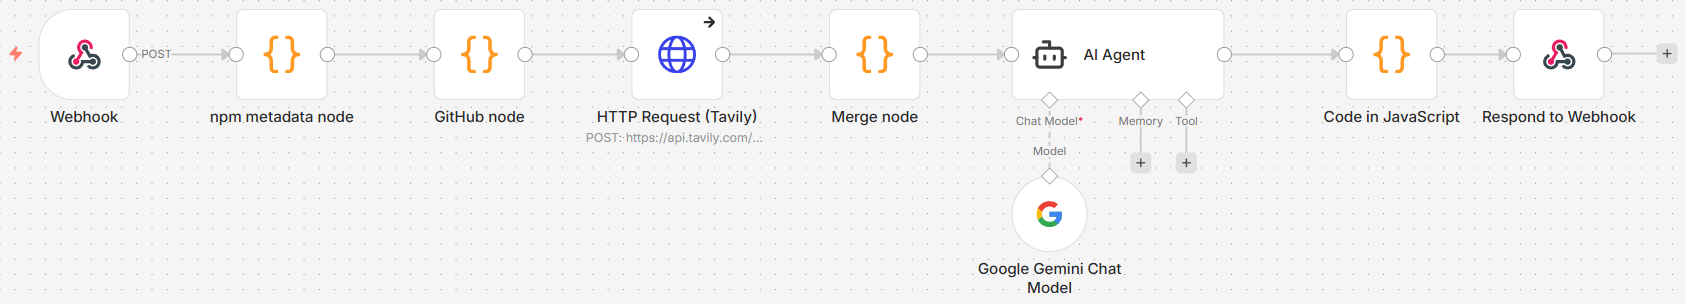
\includegraphics[width=\textwidth,keepaspectratio]{img/n8n-workflow.png}
  \caption[AI-workflow in n8n]{Overzicht van de n8n-workflow die metadata, release notes, webcontext en AI-samenvatting combineert}
  \label{fig:n8n-workflow}
\end{figure}

\subsection{Fase 4 - Vergelijkende onderbouwing van architectuur en AI-aanpak}
\label{sec:fase4}

De vierde fase richt zich op het onderbouwen en verfijnen van de gemaakte ontwerpkeuzes aan de hand van een gerichte vergelijking van de drie uitgewerkte AI-agentoplossingen en eventuele architecturale varianten. Op basis van de requirements uit fase 2 wordt een set \emph{eenvoudig meetbare} evaluatiecriteria opgesteld, zoals:
\begin{itemize}
    \item gemiddelde verwerkingstijd per update (doorlooptijd van input tot samenvatting);
    \item technische inspanning voor opzet en onderhoud (bijvoorbeeld aantal configuratiestappen, hoeveelheid code);
    \item kwaliteit van samenvattingen gemeten via een eenvoudige beoordelingsschaal door de co-promotor (bijvoorbeeld 1–5 voor duidelijkheid en relevantie);
    \item fout- of faalratio (bijvoorbeeld aantal mislukte runs of onvolledige resultaten per tien updates).
\end{itemize}

Aan de hand van een aantal representatieve scenario’s (bijvoorbeeld updates met alleen kleine bugfixes, updates met beveiligingspatches, updates met potentieel brekende wijzigingen) worden OpenAI Agent Builder, n8n en Flowise onder dezelfde omstandigheden getest en met elkaar vergeleken. De focus ligt hierbij niet op een brede marktanalyse, maar op het versterken of bijsturen van de gekozen architectuur en het bepalen welke aanpak het meest geschikt is als basis voor het verdere gebruik van het dashboard in deze specifieke use case. Deliverables van fase 4 zijn:
\begin{itemize}
    \item experimentele beschrijvingen van de uitgeprobeerde varianten;
    \item meetresultaten volgens de gedefinieerde criteria (doorlooptijd, inspanning, beoordelingsscores, foutpercentages);
    \item een gemotiveerde keuze of bevestiging van de uiteindelijke architectuur en AI-configuratie.
\end{itemize}

\subsection{Fase 5 - Evaluatie en rapportering}
\label{sec:fase5}

In de laatste fase wordt het proof-of-concept geëvalueerd met de co-promotor binnen het bedrijf, aan de hand van een combinatie van demonstraties, gericht feedbackgesprekken en, waar mogelijk, beperkte praktijktesten realistische projecten. De evaluatie focust op bruikbaarheid van het dashboard, de gemeten vermindering van manuele analysetijd (bijvoorbeeld aantal geanalyseerde updates per uur vóór en na gebruik), de door de co-promotor toegekende beoordelingsscores voor duidelijkheid van de AI-samenvattingen en de mate waarin het systeem helpt bij de prioritering van updates.

De bevindingen uit deze evaluatie worden gecombineerd met de kwantitatieve resultaten van fase 4 om de onderzoeksvragen te beantwoorden en de onderzoekshypothesen te toetsen. Deliverables van fase 5 zijn:
\begin{itemize}
    \item een synthese van de evaluatie met de co-promotor (inclusief gemeten tijdswinst, kwaliteitsbeoordelingen en verbetervoorstellen);
    \item de uitgewerkte bachelorproef met een geïntegreerde beschrijving van probleem, methode, resultaten en conclusies;
    \item aanbevelingen voor verdere ontwikkeling en mogelijke integratie van het systeem in de bredere ontwikkelprocessen van het bedrijf.
\end{itemize}

De globale fasering en tijdsplanning van het onderzoek wordt weergegeven in Figuur~\ref{fig:gantt}.

\begin{figure}[h!]
  \centering
  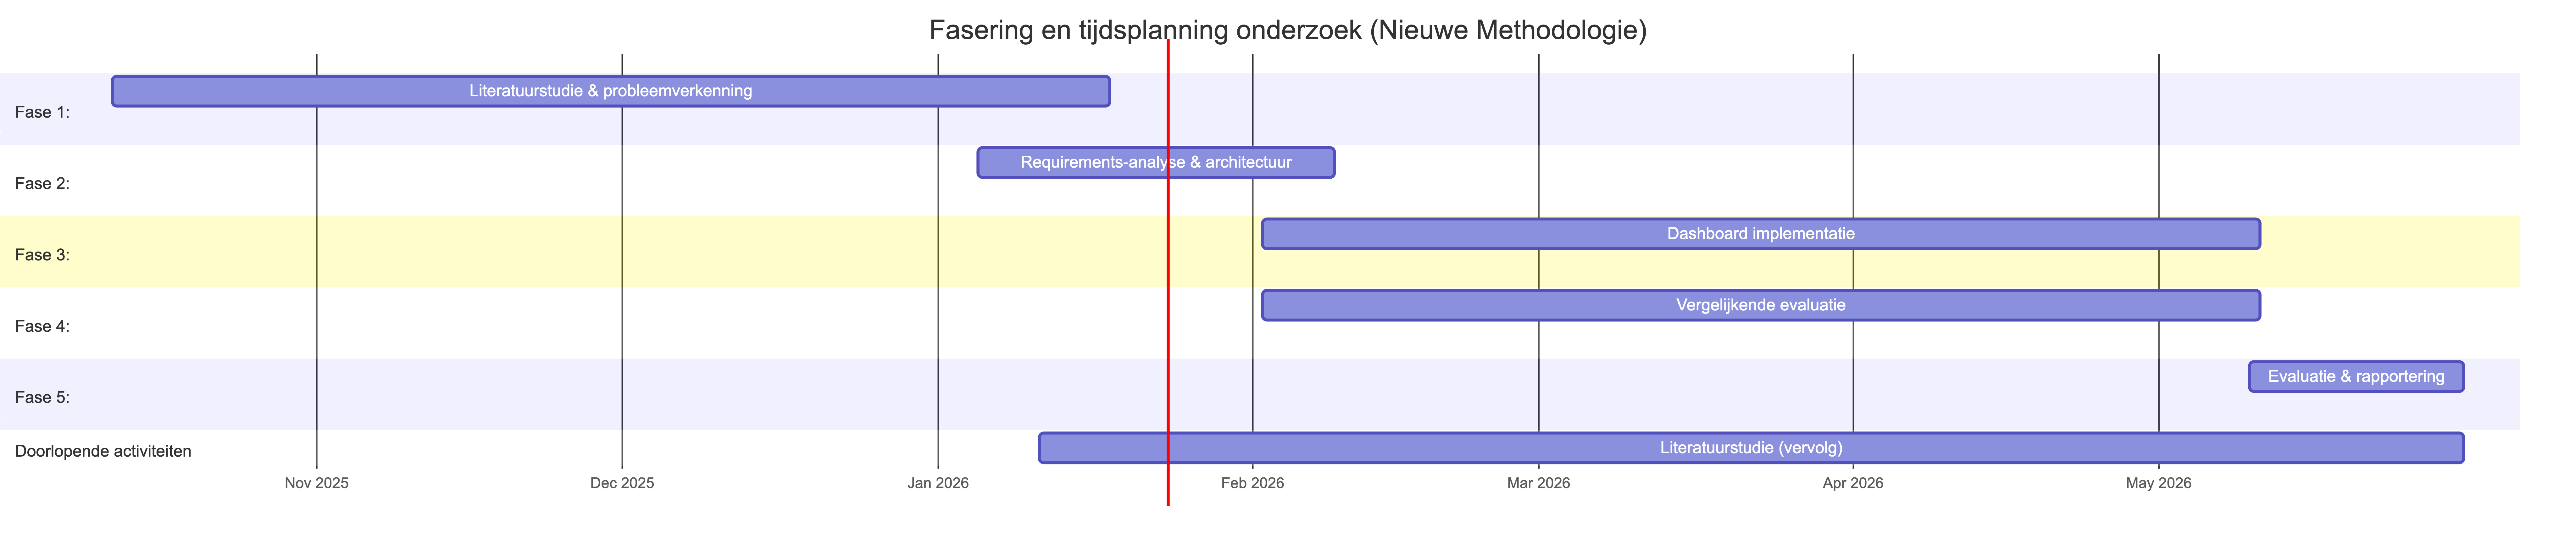
\includegraphics[width=0.85\paperwidth, keepaspectratio]{img/Figure_1.png}
  \caption{Fasering en tijdsplanning van het onderzoek}
  \label{fig:gantt}
\end{figure}

\clearpage

% \lipsum[21-25]

